%% PNAStwoS.tex

%% BASIC CLASS FILE
\documentclass{pnastwo2}

%% ADDITIONAL OPTIONAL STYLE FILES
\usepackage{graphicx}
%\usepackage{pnastwoF}
\usepackage{amssymb,amsfonts,amsmath}
\usepackage{caption}
\usepackage{subcaption}
\usepackage{float}
\usepackage{wrapfig}
\usepackage{caption}
\usepackage{cite}
%% OPTIONAL MACRO DEFINITIONS
\def\s{\sigma}

%%%%%%%%%%%%
\url{http://cs230.stanford.edu/}
\copyrightyear{2019}
\issuedate{CS 230}
\volume{Winter 2019}
%%%%%%%%%%%%

\begin{document}

\title{Making yourself into a work of art}

\author{Kiah Hardcastle\affil{1}{Neurosciences Program}
\and Julie Makelberge\affil{2}{Graduate School of Business, Stanford University}}

\contributor{Project Milestone for CS 230: Deep Learning, February 2019}

\maketitle

\begin{article}

\begin{abstract}

In this paper, we outline the implementation of a neural style transfer framework that will integrate a person's face in an artistic painting. For example, given a headshot and a picture of the Mona Lisa, this framework would inpaint the headshot face into the face of the Mona Lisa, while retaining the artistic style of the Mona Lisa. There are a number of existing applications that have focussed face swapping in recent years, however they have generally focussed on doing so for photograph images. Furthermore, the few methodologies that have used neural style transfer to adjusting such photos to an artistic style, have constrained their solution to well-aligned images that contain only a face (i.e., cropped images), without taking into account the pose of the face. Our approach is novel in that we aim to retaining the style and pose of the original work of art's face, regardless of the pose of the supplied image, and will reintroduce the face in the work of art as a whole. 

\end{abstract}

\dropcap{N}eural style transfer is the technique of using deep neural networks to transfer the style of a given reference image to the content of another. Traditionally, such problems have been adressed with classic image processing techniques such as histogram matching \cite{neumann2005color}. However, in 2015 Gatys et all. \cite{gatys2015neural} introduced a novel technique that leverages the power of Convolutional Neural Networks to emulate famous painting styles in natural images. In their seminal paper, they proposed to use the encoding from different layers of a pre-trained CNN, to capture the style elements and content elements of images. They then used an interative approach to optimise an image with the objective of minimizing the distance between the style elements of the image and the reference work of art, while keeping changes to the content as small as possible. 
\par
Their work has inspired a number of new neural transfer algorithms, ranging from general models such as the work of Li and Wand \cite{li2016combining} that combined generative Markov random field models with deep convolutional neural networks, to highly specialised domain-specific models such as Jiang anf Fu's Fashion style generator \cite{jiang2017fashion}. While general models have shown great potential in a large number of applications, they have generally introduced visual artifacts which are especially striking in faces, given human's sensitivity for facial irregularities. The work of Selim et all. \cite{selim2016painting} introduced the first approach for single-example based head portrait painting not constrained to a specific style. Their approach was successful by introducing additional constraints that exploit human facial geometry through the notion of gains maps. However, their methodology focused on front-facing cropped facial images and does not yet generalise to different facial positions or introduction within the wider context of a full painting. 
\par
In this work, we aim to expand on the work of Selim et all by introducing a framework that combines different Neural Transfer techniques to tackle the challenge of introducing faces of slightly varing positions in a work of art. Our goal is to create a resulting image that looks similar to our reference work of art, but with the exception of having a different person in mind at the time of painting. This technique would be valuable in the world of generative art as it alows different and personalised renderings of the same types of art work. 

\section{Approach and Results}

We have broken down our framework in a number of steps. First, we must identify the region containing the face in both images (art image = image A with face A, other image = image B with face B). Note that we assume that images with only one face are considered, or in images with multiple faces we would only consider the most prominent one. Once faces A and B are identified and cropped out of the images, we must then align the faces to be in similar positions. Specifically, we require that face B be in the same pose, or alignment, as face A in our reference work of art. Using the aligned faces, we then generate a new face B', using neural style transfer (or visual attribute transfer, see below). Here, face B' contains the content of face B, in the style of face A. Next, we will replace face A with the new face B' in our reference work of art. Finally, we will smooth the boundaries between the excised region surrounding face B' and the rest of the image.

\subsection{Data collection}

Fortunately, as many of our methods will rely on pre-trained networks, we do not need large numbers of new images with which to train our network. However, there are large open-source datasets of artwork and faces available on the internet, which we plan to take advantage of in order to demonstrate our approach. To generate our dataset of artwork, we use the Web Gallery of Art \cite{WebGallery}. This dataset is free to use for educational purposes and contains the meta data and links to images for more than 45,000 works of art, 31,000 of which are paintings. In order to create the dataset, we wrote write a script to download these images (see github repo).  To generate a dataset of faces, we initially plan to use own headshots. However, we plan to use the celebA dataset \cite{liu2018large} if more face images are required.

\subsection{Data pre-processing: face-cropping}

The first step in our pipeline is to identify the face in both images (image A and image B), and generate new images A' and B', which are the cropped-out face of images A and B respectively. To accomplish this, we implemented an open-source face recognition from the OpenCV package. Following the procedure detailed in the Medium blogpost \cite{Medium}, we used Haar Feature-based Cascade Classifiers to detect the bounding box of the face. In brief, Haar features are similar to the filters in a CNN, but different in that they are not learned during training - they are pre-determined. Each filter can be used in a classifier to determine whether or not a face is present in a bounding box of the image. While the classification based on one Haar filter is not great, combining the output of many filters (e.g. through boosting) will return a relatively good classification. The OpenCV implementation organizes the features into a cascade, so that a lot of filters are "tried" if the image within the bounding box seems promising (i.e. early filters classify the image as a face). The OpenCV implementation contains pre-trained filters for faces, which we can load and then use to detect face regions within an image (see code in the github). An example of an output of the model is given below in Figure 1:

\begin{figure}[ht]
	\begin{center}
		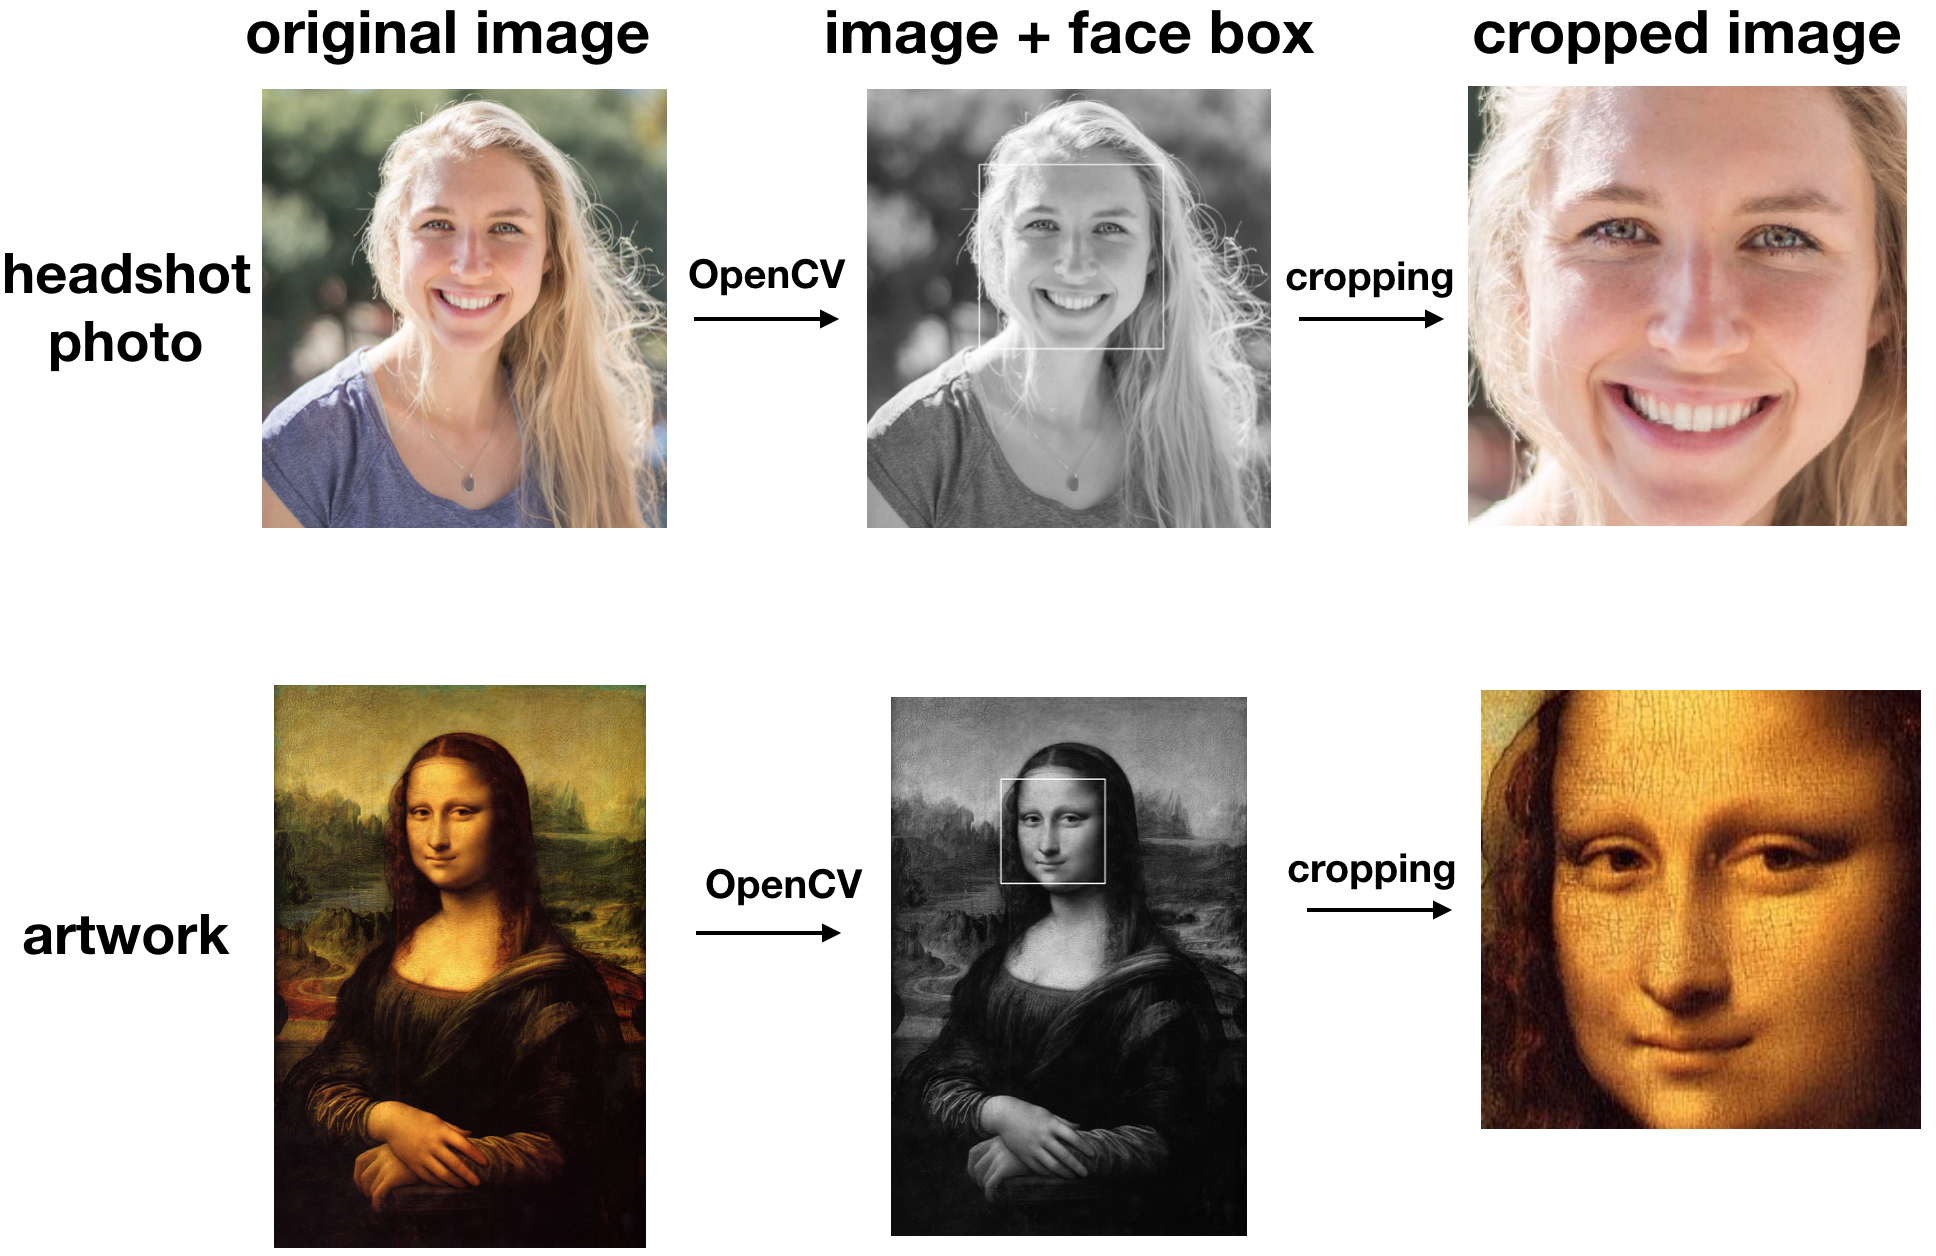
\includegraphics[width=.45\textwidth]{face_crop_figure}
		\caption{Examples demonstrating face cropping pipeline.} \label{fig:face_crop}
	\end{center}
\end{figure} 

\subsection{Data pre-processing: face-alignment}

The second step in our pipeline is to properly align the faces so that the pose of the face is similar between the two images. Specifically, we want face B to be in the same pose as face A - e.g. the major face landmarks (eyes, nose, mouth, chin) should be in similar locations. To accomplish this, we must first identify important landmark features in both images, and then apply a transformation to get face B in the same pose as face A. In order to identify salient landmarks, we used the dlib face detection and landmark identification package, and based our code off of a github repository \cite{dlib}. An example of the output of this procedure is given below:

\begin{figure}[ht]
	\begin{center}
		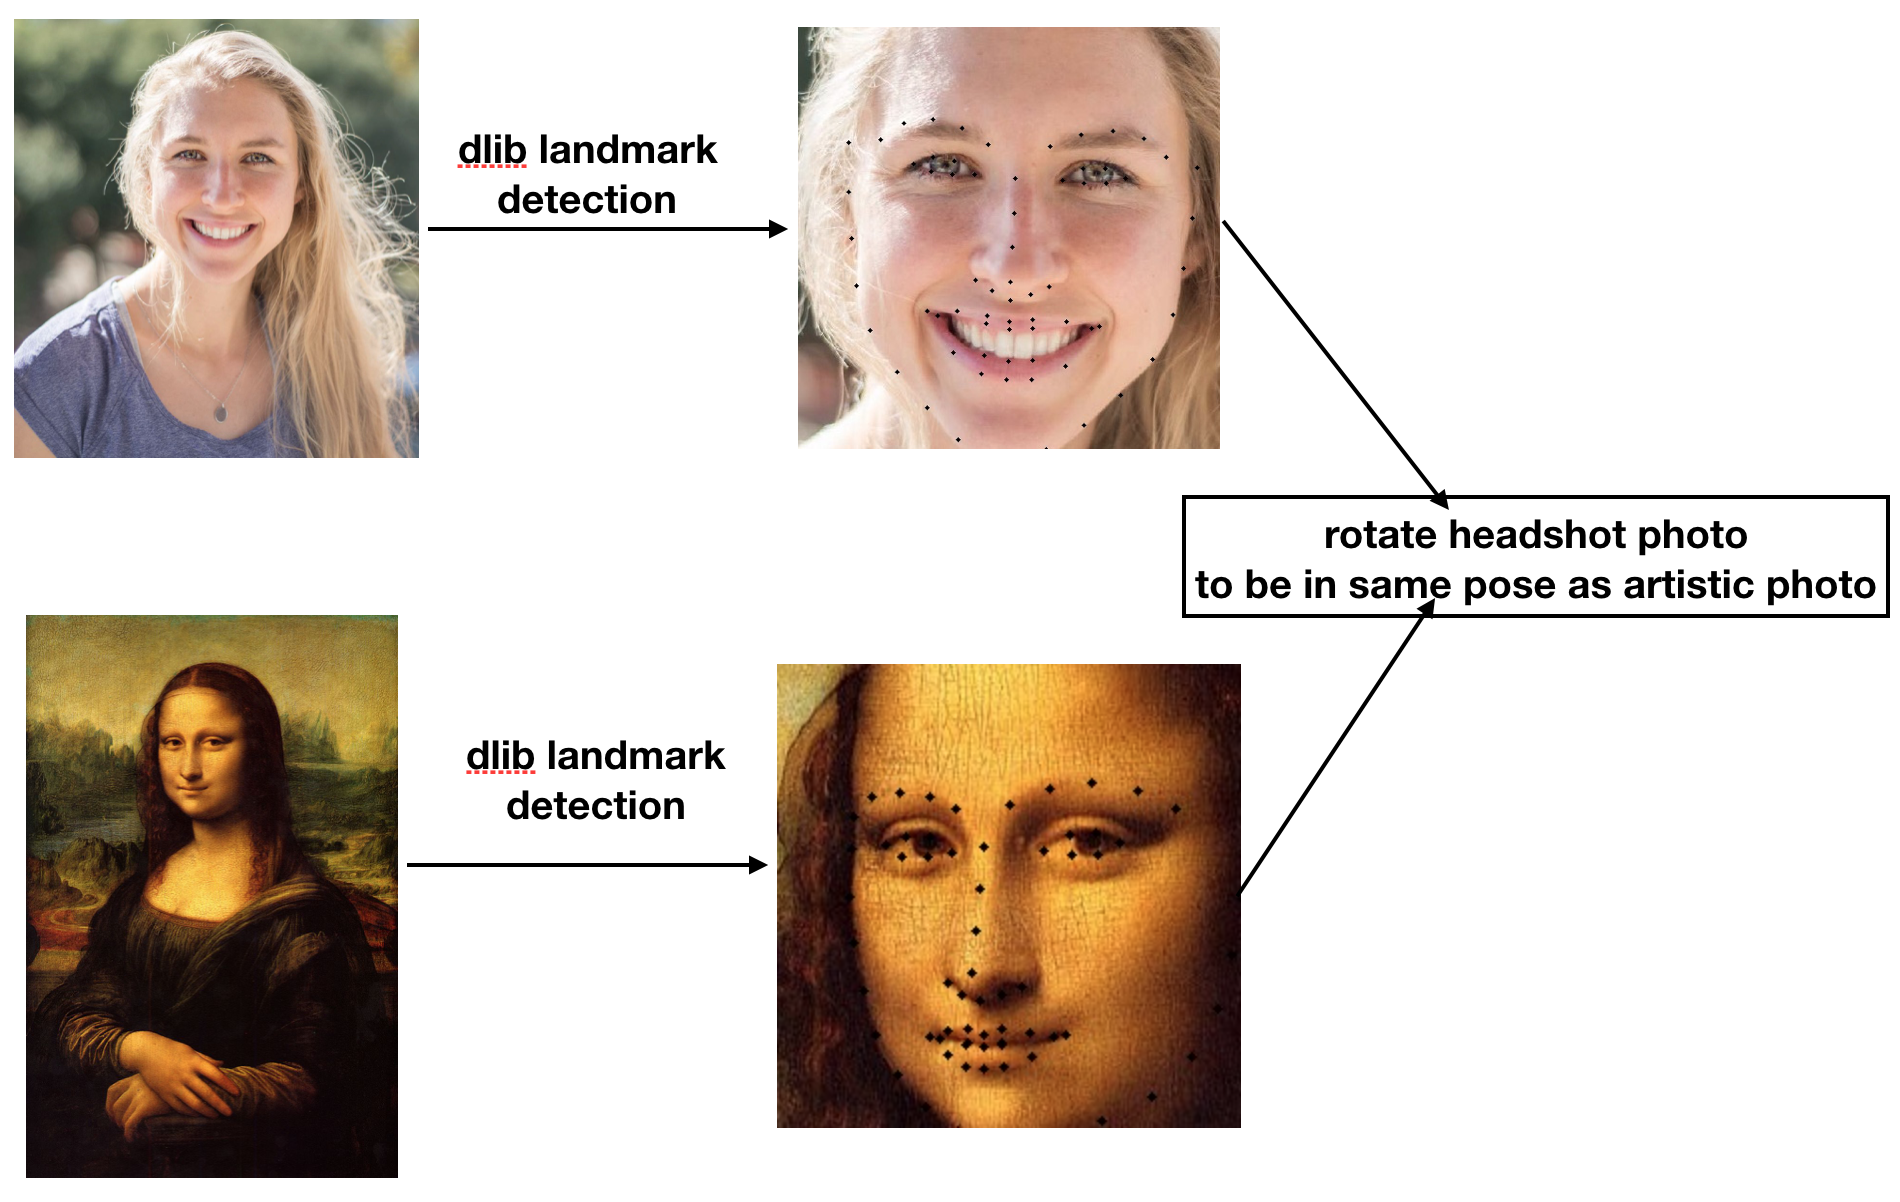
\includegraphics[width=.4\textwidth]{landmark_id}
		\caption{Face alignment pipeline with example landmark detection.} \label{fig:nst}
	\end{center}
\end{figure} 

We will then implement a function that will transform the headshot photo into the same pose as the artistic photo by applying a transformation that will align the landmark points. While we have not completed this yet, we plan on completing this step for our final deliverable. There are some previous implementations of this task, including one found in the Face Alignment in Full Pose Range paper by Xiangyu Zhu et al. \cite {zhu2019face}

\subsection{Style transfer between face images}

The third step in our pipeline is to generate a new image B' that contains the content of face B (the non-artistic face) in the style of face A (the artistic face). There are several possible methods to accomplish this task. One simple method would be to use Neural Style Transfer in a manner similar to the Coursera CNN module homework, or using another implementation of Neural Style Transfer. While this method is not face specific, and thus may not perform very well, it is a good straight-forward approach to implement and further iterate on. A second method would be to follow the algorithm defined in the paper "Visual Attribute Transfer through Deep Image Analogy", by Jing Liao et al \cite{liao2017visual}. This method differs from traditional Neural Style Transfer in that it focuses on creating a pixel by pixel mapping based on higher level features between the images, among other differences. Finally, a third method would be to follow the algorithm described in the paper "Painting Style Transfer for Head Portraits using Convolutional Neural Networks" by Selim et al. \cite{} In this method, they use network trained on faces specifically, and so the style transfer is targeted towards head portraits.

While ultimately we feel that the third method is the most promising, as it is focused on style transfer of portraits, thus far we have focussed on more traditional neural style transfer on the cropped images of face A and face B given our time constraints and the availability of pre-trained CNN weights. We are currently working with two implementations of Neural Style Transfer. In the first, we altered the code that was used in the Coursera course to perform neural style transfer on our two images. In this method, we generate a new image B' with the content of face B and in the style of face A. To do this, we minimize the following loss function:
\[
J(G)=\alpha J_{content}(B,B')+\beta J_{style}(A,B')
\]
where
\[
 J_{content}(B,B') = \frac{1}{4n_Hn_Wn_H} \sum_{all} (a(A) - a(B'))^2
\]
and 
\[
 J_{style}(B,B') = \sum_l  \lambda_l \frac{1}{(2n_Hn_Wn_H)^2} \sum_{ij} (B'_{ij}(A)^{(l)} - B'_{ij}(B')^{(l)})^2
\]

where $a(A)$ are the activations of single layer of a pre-trained VGG-19 network with the content image as input, $a(B')$ are the activations of the same layer of the VGG-19 network with the newly generated image put through, $B'_{ij}(S)^{(l)}$ is the Gram matrix of activations of a single layer ($l$) of the same network when the style image is used as input, and finally $B'_{ij}(G)^{(l)}$ is the Gram matrix of activations of a single layer of the same network when the newly generated image is used as input. Minimizing this loss function by altering the pixels in the generated image will result in a new image that contains the content of the content image, and the style of the style image. 

While we were able to successfully perform neural style transfer using our code from the homework, we found another implementation of the same algorithm that gave us a much better output \cite{NeuralStyleTranferGithub}. The result of this implementation is shown below in Figure 3:

\begin{figure}[ht]
	\begin{center}
		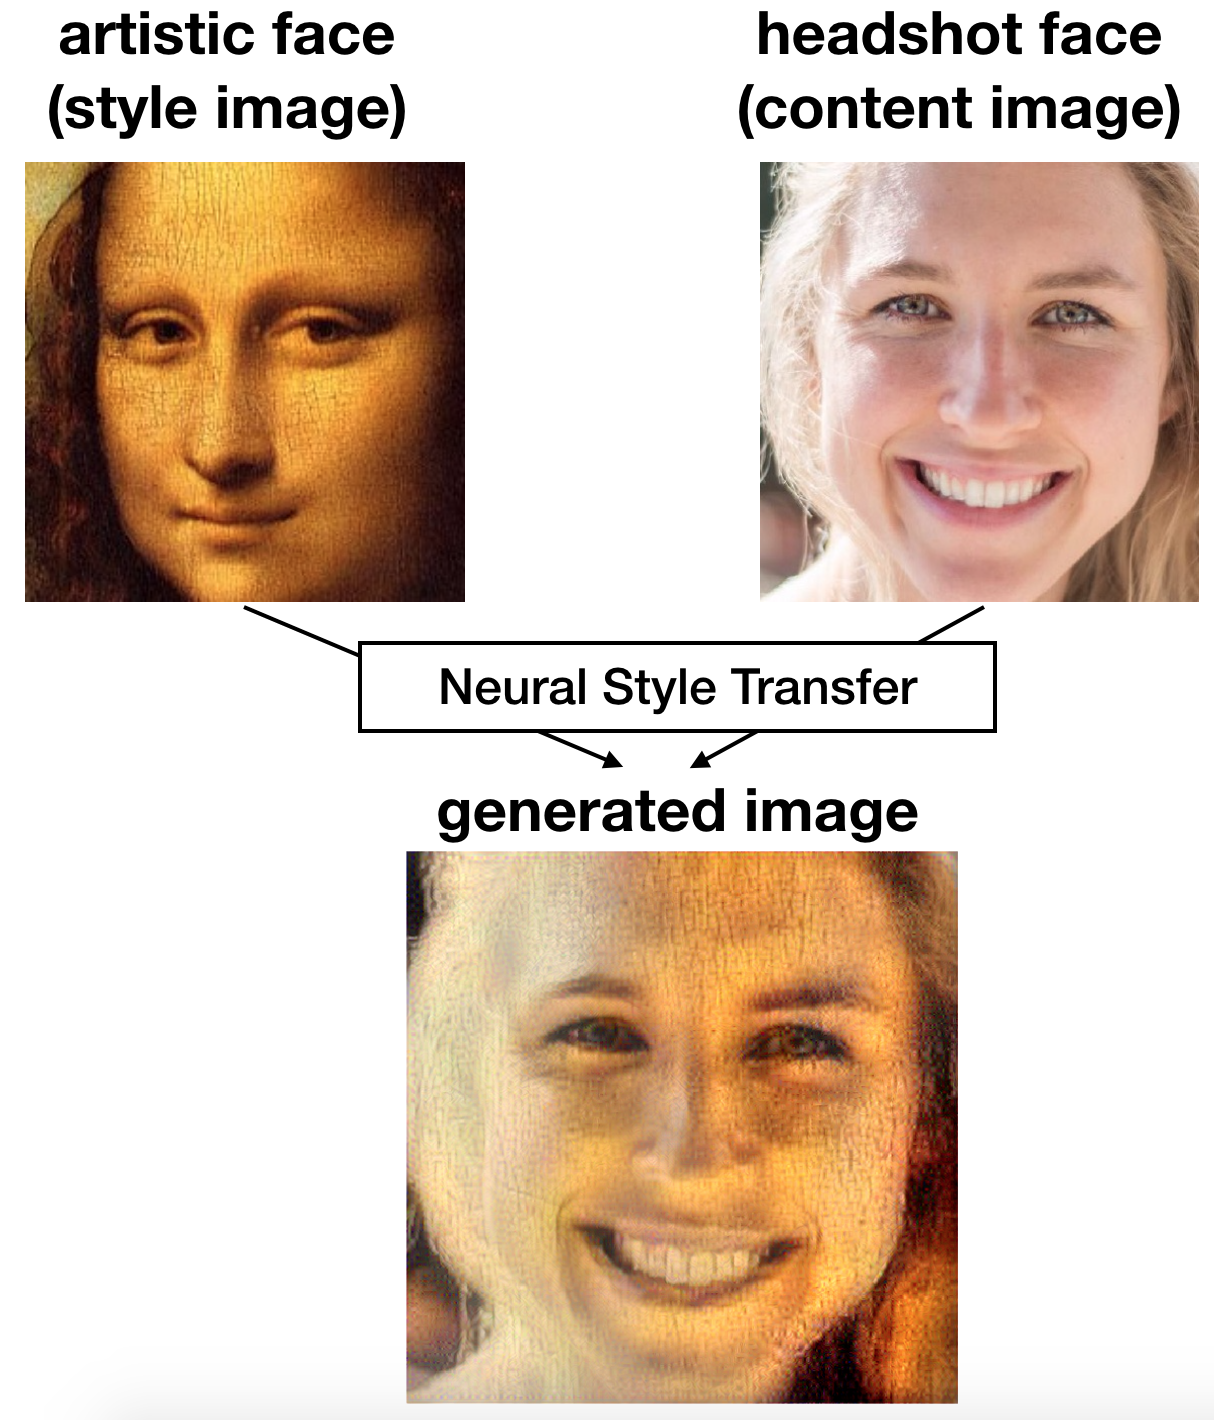
\includegraphics[width=.4\textwidth]{neural_style_transfer_output_v2}
		\caption{Example output using Neural Style Transfer.} \label{fig:nst}
	\end{center}
\end{figure} 

\subsection{Face-replacement in artistic image}

Finally, we must replace the original face A with the new, properly aligned face C. This task contains two components: first, we replace the pixels within the original bounding box in image A with the new image B'. Second, we must then smooth the boundary between in the inpainted pixels and the border. The first step of this procedure is quite easy. To do the second step, we will remove the area around the bounding box of the face (i.e. the boundary between the new image and the old image), and then use methods of inpainting in order to fill in the boundary. 

\section{Summary}

In summary, successful completion of our project will require identifying faces in two images, cropping the faces out, aligning the faces, performing style transfer to generate a new face image, replacing the artistic face with the newly generated face, and smoothing the edges so the artistic image looks similar (except for the face) to the original. Thus far, we have been able to identify faces in images, crop them out, did the first step in aligning the faces, and performed neural style transfer. To finish the project, we plan on first working on aligning the faces, replacing the image with correct smoothing and inpainting if need be, and finally improving our neural style transfer by trying other implementations or by varying hyperparameters and training time in our current implementations.

\section{Code}

All code for the project, and in fact everything for the project, can be found in the following github repository: https://github.com/khardcastle/face-in-art.


\begin{acknowledgments}
We thank Andrew Ng and Kian Katanforoosh for teaching us the techniques used in this project, and to our project TA Kaidi Cao for guiding us towards workable solutions for our problem and pointing us to relevant literature.
\end{acknowledgments}

\bibliography{References}
\bibliographystyle{plain}


\end{article}
\end{document}